
\subsection{Zeichenfläche}

\subsubsection{Aufgaben}
Die Software soll dem Anwender ermöglichen in einer Zeichenfläche eine einfache Zeichnung zu erstellen. Dazu stehen im einige Werkzeuge zum Zeichnen von Quadraten, Kreisen und Linien zur Verfügungn. Es soll jedoch auch möglich sein freihändig zu zeichnen, wodurch der Benutzer frei nach seinen Wünschen ein Bild malen kann. Die fertige Zeichnung soll anschließend automatisch in Befehle für den Roboter übersetzt werden, welcher die Figur nachzeichnet.

\subsubsection{Aufbau}
Für diese Aufgabe wird ein eigenes Control, das DrawingCanvas, basierend auf dem InkCanvas von WPF, sowie Teile der Edubot-API verwendet. Das InkCanvas ermöglicht dem Benutzer das Erstellen von Freihandzeichnungen und kann sogar bestimmte Gestiken erkennen. Da diese Funktion in unserer Applikation jedoch nicht benötigt wird, haben wir uns nicht näher damit beschäftigt. Welche Aktion nun ausgeführt wird, wenn der Benutzer in das InkCanvas klickt, hängt von der Eigenschaft InkCanvasEditingMode ab, welche folgende Werte annehmen kann:
\begin{itemize}
\item EraseByPoint - Ermöglicht das Löschen einzelner Punkte
\item EraseByStroke - Ermöglicht das Löschen einzelner Pinselstriche, welche im weiteren Kontext auch Strokes, genannt werden. Ein Pinselstrich sind alle Punkte die ein Benutzer in einem Durchzug zeichnet.
\item GestureOnly - Ermöglicht das Erkennen von Gestiken
\item Ink - Ermöglicht das Erstellen von Freihandzeichnungen
\item InkAndGesture - Ermöglicht das Erstellen von Freihandzeichnungen und das Erkennen von Gestiken.
\item None - Es wird keine Aktion ausgeführt
\item Select - Ermöglicht das Selektieren und Löschen von Pinselstrichen
\end{itemize}
In der Anwendung kommen die Modi EraseByPoint, EraseByStroke, Ink und Select zum Einsatz. Die Selektion letzterer erfolgt über eine, links vom InkCanvas befindliche, Werkzeugleiste. Um dem Benutzer das Zeichnen von Kreisen, Rechtecken und Linien zu ermöglichen wird eine eigene Enumeration mit Namen InkCanvasDrawingMode verwendet. Diese beinhaltet folgende Werte:
\begin{itemize}
\item Line - Ermöglicht das Erstellen von Linie
\item Rectangle - Ermöglicht das Erstellen von Rechtecken
\item Ellipse - Ermöglicht das Erstellen von Ellipsen
\end{itemize}
Der vordefinierte Modus None kommt hierbei auch indirekt zum Einsatz, da er indiziert ob der Benutzer gerade eine der oben erwähnten geometrischen Figuren zeichnet. 
Da die Zeichenfläche zur schnelleren Verwendung auch die Undo/Redo-Funktion unterstützen sollte, wurde in unserem Control das Memento-Pattern verwendet. Außerdem soll die Zeichenfläche das Einzeichnen von, durch den aktuell verwendeten Adapter, nicht erreichbaren Punkten verhindern. Um den Arbeitsbereich auch visuell darzustellen umrandet das DrawingCanvas den gültigen Bereich mit einer grauen Linie.

\subsubsection{Bedienung der Oberfläche}

\begin{figure}[H]
  \centering
  \begin{minipage}[t]{12 cm}
  	\centering
  	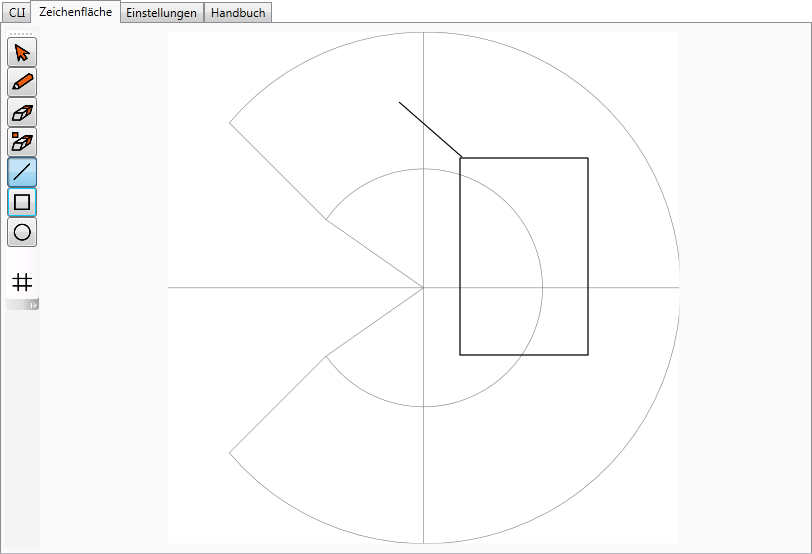
\includegraphics[width=12cm]{images/DrawingArea} 
    \caption{Die Zeichenfläche}
  \end{minipage}
\end{figure}

Um die Zeichenfläche zu nutzen, kann der Benutzer im linken Bereich des Tabs ein entsprechendes Werkzeug durch einen Klick auswählen. Anschließend kann er, wie aus anderen Zeichenanwendungen bekannt, die gewünschten Linien, Punkte und Formen einzeichnen. Die einzelnen Werkzeuge werdne im folgenden erläutert:
\begin{itemize}
\item \textbf{Auswahl}: Wenn dieses Werkzeug ausgewählt wird, können Strokes (siehe Umsetzung für nähere Erklärung) ausgewählt und verschoben beziehungsweise über die Entfernen-Taste gelöscht werden.
\item \textbf{Freihand}: Wenn dieses Werkzeug ausgewählt wird, kann innerhalb der Zeichenfläche freihändig gezeichnet werden
\item \textbf{Radiergummi}: Wenn dieses Werkzeug ausgewählt wird, können beliebige Ausschnitte der Zeichnung gelöscht werden
\item \textbf{Stroke-Radiergummi}: Wenn dieses Werkzeug ausgewählt wird, können ganze Strokes mit einem Mausklick gelöscht werden
\item \textbf{Lineal}: Wenn dieses Werkzeug ausgewählt wird, können mittels "'Drag and Drop"' Linien in der Zeichenfläche gezeichnet werden
\item \textbf{Rechteck}: Wenn dieses Werkzeug ausgewählt wird, kann mittels "'Drag and Drop"' ein Rechteck gezeichnet werden
\item \textbf{Ellipse}: Wenn dieses Werkzeug ausgewählt wird, kann mittels "Drag and Drop" eine Ellipse gezeichnet werden
\end{itemize}

\subsubsection{Umsetzung der Zeichenfunktion}

DrawingCanvas
Wie im Aufbau erwähnt, wird dazu das, von InkCanvas abgeleitete, DrawingCanvas-Control verwendet. Im Konstruktor der Klasse werden zunächst die Methoden SetOrigin, UpdateShape und AddStrokes an verschiedene Mausbewegungen gebunden und der EditingMode auf InkCanvasEditingMode.Select gesetzt. Weiters wurde das Property IsDrawingShape definiert, welches angibt ob der Benutzer gerade eine geometrische From zeichnet. Dazu wird lediglich geprüft ob der EditingMode auf InkCanvasEditingMode.None gesetzt ist und entsprechend ein Wert vom Typ Boolean zurückgeliefert. Weiters besitzt das DrawingCanvas ein Property DrawingMode vom Typ InkCanvasDrawingMode, welches definiert welche geometrische Form der Benutzer gerade zeichnet.
\begin{itemize}
\item \textbf{SetOrigin}\\
Die Methode SetOrigin wird aufgerufen, wenn der Benutzer die linke Maustaste drückt während sich der Mauszeiger im DrawingCanvas befindet. Da Methode nur benötigt wird, um geometrische Formen zu zeichnen wird zuerst das IsDrawingShape-Property überprüft. Liefert letzteres true zurück, so wird der aktuelle Punkt in der globalen Variable origin vom Typ Point gespeichert.
\item \textbf{UpdateShape}\\
Die Methode UpdateShape wird aufgerufen, wenn der Benutzer den Mauszeigen innerhalb des Controls bewegt. Auch hier wird zuerst das IsDrawingShape-Property überprüft. Ist dieses auf true gesetzt, so wird die InvalidateVisual-Methode aufgerufen, welche das DrawingCanvas neu zeichnet. Dazu ruft WPF die OnRender-Methode der Klasse auf, in welcher geprüft wird ob gerade eine geometrische Form gezeichnet wird und um welche es sich handelt. Abhängig von diesen Faktoren wird mit Hilfe eines DrawingContext-Objekt die entsprechende Form gezeichnet.
\item \textbf{AddStrokes}\\
Die Methode AddStrokes wird aufgerufen, wenn der Benutzer die linke Maustaste loslässt. Zuerst wird erneut das IsDrawingShape-Property geprüft und anschließend die aktuelle Position des Mauszeigers gespeichert. Da wir nun über den Ausgangspunkt, repräsentiert durch die origin-Variable, als auch den Endpunkt currentPoint verfügen, ist die Größe der geometrischen Form definiert.
Mit Hilfe einer switch-Kontrollstruktur wird nun ermittelt, welche Form der Benutzer gezeichnet hat und ein entsprechendes Stroke-Objekt erzeugt. Ein Stroke enthält eine Menge an Punkten, die sogenannten StylusPoints, welche, wenn das Objekt zur Stroke-Collection der InkCanvas-Klasse hinzugefügt wird, gezeichnet werden. Zwischen den angegebenen Punkten wird jeweils eine Linie gezeichnet, wodurch ein Stroke-Objekt mit entsprechend definierten Punkten eine geometrische Form darstellen kann.
\end{itemize}

\textbf{Umrechnung der geometrischen Formen in Strokes}
Wie oben erwähnt, findet in der AddStrokes Methode die Umrechnung der, vom Anwender gezeichneten Form, in entsprechende Strokes statt. 
\begin{itemize}
\item \textbf{Line}\\ 
Hierbei wird ein Stroke-Objekt mit zwei StylusPoints, dem Ursprungs- und dem Endpunkt, generiert.
\item \textbf{Rectangle}\\ 
Hierbei wird ein Stroke-Objekt mit fünf StylusPoints generiert. Die Zusammenstellung dieser Punkte kann der folgenden Grafik entnommen werden.
\begin{align}
P_1 = (x_{origin} / y_{origin})\\
P_2 = (x_{currentPoint} / y_{origin})\\
P_3 = (x_{currentPoint} / y_{currentPoint})\\
P_4 = (x_{origin} / y_{currentPoint})\\
P_5 = (x_{origin} / y_{origin})
\end{align}

\item \textbf{Ellipse}\\ 
Hierbei wird ein Stroke-Objekt mit einer, von der Ellipsengröße abhängigen, Menge an StylusPoints generiert. Zur Berechnung der Ellipsenpunkte kommt ein ähnliches Verfahren wie bei zirkularen Interpolation zum Einsatz.
\begin{enumerate}
\item Radien der Ellipse berechnen\\
Zuerst müssen die zwei Radien der Ellipse $r_x$ und $r_y$ mit Hilfe des Ursprungs- und des Endpunkts berechnet werden.
\begin{align}
r_x &= x_{origin} - x_{currentPoint}\\
r_y &= y_{origin} - y_{currentPoint}
\end{align}
\item Anzahl der Ellipsensegmente ermitteln\\
Anschließend wird die ungefähre Anzahl der zu berechnenden Außenpunkte mit folgender Formel berechnet.
\begin{align}
n = 4 \sqrt{r_x^2+r_y^2}
\end{align}
\item Winkelsteigung berechnen\\
Im nächsten Schritt wird die Steigung des Winkels pro berechnetem Punkt kalkuliert.
Anmerkung: Da die Math.Sin beziehungsweise Math.Cos-Methode nur einen Winkel in Radiant übernimmt, wird hier in der Anwendung $\frac{2\pi}{n}$ gerechnet.
\begin{align}
k_{\theta} = \frac{360^\circ}{n}
\end{align}
\item Mittelpunkt berechnen\\
Nun wird der Mittelpunkt, erneut mit Hilfe des Ursprungs- und Endpunkts, berechnet.
\begin{align}
m_x &= x_{origin} + r_x\\
m_y &= y_{origin} + r_y
\end{align}
\item Berechnung der Außenpunkte\\
Zuerst wird ein Startpunkt für die weitere Berechnung festgelegt, welcher wie folgt definiert ist:
\begin{align}
s_x &= m_x + r_x\\
s_y &= m_y
\end{align}
Anschließend werden in einer Schleife die Zwischenpunkte berechnet und als als StylusPoints zum Stroke hinzugefügt. Der $i$-te Zwischenpunkt, definiert durch $p_x$ und $p_y$, wird nach folgender Formel berechnet:
\begin{align}
p_x &= m_x + r_x \cos(ik_\theta)\\
p_y &= m_y + r_y \sin(ik_\theta)
\end{align}
\end{enumerate}

\item
\end{itemize}
Vor dem Hinzufügen des Strokes wird geprüft ob er StylusPoints enthält, da es in Ausnahmefällen dazu kommen kann das keine Punkte berechnet wurden. Ein Beispiel für einen solchen Ausnahmefall wäre eine Ellipse mit Radius 0, welche durch einen versehentlichen Klick in die Zeichenfläche berechnet wird. Enthält der Stroke jedoch Punkte, so wird er über das OnStrokeCollected-Events, verpackt in einem StrokeCollectedEventArgs-Objekt, der Stroke-Collection des InkCanvas hinzugefügt. 

\subsubsection{Umsetzung der Undo/Redo-Funktion}
Um Aktionen innerhalb der Zeichenfläche rückgängig beziehung wiederholbar zu machen, wird das sogenannt Memento-Pattern verwendet. Letzteres ist eine Software-Architektur-Muster, welches von der "'Gang of Four"', einer Gruppe von Programmierern, für spezielle Aufgaben entwickelt wurde. Das Memento-Pattern eignet sich hervorragend für Aufgaben wie Undo/Redo-Operationen, weshalb es in der DrawingCanvas-Klasse verwendet wird.\\
Die Idee dahinter ist, dass für jede Operation ein sogenanntes Memento erzeugt und einer chronologisch geordneten Liste hinzugefügt wird. Das Memento enthält genauere Informationen über die ausgeführte Operation. Durch Iteration der Liste können alle von Beginn an durchgeführten Operationen nachvollzogen werden.\\
\\
Im Falle des DrawingCanvas enthält ein Memento folgende Properties:
\begin{itemize}
\item Operation\\
Das Operation-Property ist vom Typ String und definiert ob ein Stroke hinzugefügt oder gelöscht wurde. Dabei steht "add" für Hinzufügen und "del" für Löschen.
\item Stroke\\
Das Stroke-Property beinhaltet den, von der Operation betroffenen, Stroke. Dadurch kann das entsprechende Objekt einfach aus der Stroke-Collection des InkCanvas entfernt beziehungsweise hinzugefügt werden.
\end{itemize}

Die Mementos werden in zwei Stacks, dem undoBuffer und dem redoBuffer, verwaltet. Ein Stack, auch Kellerspeicher genannt, stapelt mit Hilfe der Push-Methode hinzugefügte Elemente übereinander beziehungsweise gibt bei Aufruf der Pop-Methode das zuletzt hinzugefügte Element zurück und entfernt dieses aus dem Stapel.\\
Um ein Memento hinzuzufügen wurde die Methode AddMemento im DrawingCanvas implementiert und im Konstruktor der Klasse dem StrokeCollected- beziehungsweise StrokeErased-Event zugewiesen. Diese Events werden beim Zeichnen und Löschen von Pinselstrichen oder Punkten ausgelöst. Die Klasse merkt sich die durchgeführte Operation durch ein neues Memento und kann diese bei Bedarf rückgängig machen, wozu lediglich eine entsprechende Gegenoperation durchgeführt wird.
\begin{itemize}
\item \textbf{AddMemento}\\
Die Methode AddMemento übernimmt als Parameter ein object sender, welches das Objekt enthält, dass das Ereignis verursacht hat, sowie ein Objekt vom Typ EventArgs mit näheren Details zum Ereignis. Bei Aufruf dieser Methode wird zuerst die globale Variable addMemento geprüft, welche angibt ob ein Memento für diese Operation hinzugefügt werden soll. Der nähere Zweck dieser Variable wird in der Undo beziehungsweise Redo-Methode beschrieben. Ist addMemento auf true gesetzt, so wird geprüft um welche spezifische Klasse es sich beim EventArgs-Objekt handelt.\\
Handelt es sich dabei um ein InkCanvasStrokeCollectedEventArgs-Objekt so indiziert dies, das ein neuer Stroke hinzugefügt wurde. Anschließend wird ein Memento mit der Operation "add" und dem, in den Event-Argumenten enthaltenen, Stroke erzeugt und in den redoBuffer gegeben. Sollte es sich beim EventArgs-Objekt um ein InkCanvasStrokeEraseEventArgs-Objekt handeln, so wird im erstellten Memento "del" als Operation angegeben. Zuletzt wird noch der redoBuffer geleert, da der Benutzer eine neue Aktion durchgeführt und deshalb die Mementos über zuvor rückgängig gemachte Aktionen verworfen werden müssen.
\item \textbf{Undo}\\
Die Methode Undo überprüft zuerst ob sich Elemente im undoBuffer befinden. Sollte dies der Fall sein, so wird das oberste Memento im Stapel entfernt und das Operation-Property überprüft. Wenn "add" als Operation angegeben wurde, so muss der entsprechende Stroke gelöscht werden, um die Aktion rückgängig zu machen. Dazu wird die Remove-Methode der Strokes-Collection mit dem, im Memento gespeicherten, Stroke aufgerufen. Handelt es sich bei der Operation um "del", so wird der betroffene Stroke mit Hilfe der Add-Methode der Strokes-Collection wieder hinzugefügt. Zuletzt wird die soeben rückgängig gemachte Aktion zu unserem redoBuffer hinzugefügt, um sie bei Bedarf wiederholen zu können.\\
Das manuelle Bearbeiten der Strokes-Collection führt erneut zu StrokesCollected beziehungsweise StrokesErased-Events, weshalb auch unsere AddMemento-Methode aufgerufen wird. Da wir in diesem Fall jedoch nicht erneut ein Memento erzeugen wollen, setzen wir vor Hinzufügen und Löschen von Strokes die addMemento-Variable auf false. Erst nach Abschluss aller Aktionen in der Undo-Methode wird diese Variable wieder auf true gesetzt und neue Mementos erzeugt. 
\item \textbf{Redo}\\
Die Methode Redo überprüft zuerst ob sich Elemente im redoBuffer befinden. Anschließend wird das oberste Memento aus dem Stapel geholt und die, im Operation-Property gespeicherte, Aktion ausgeführt. Hierbei kommen dieselben Methoden wie in der Undo-Methode zum Einsatz, nur das hierbei die im Memento angegebene Operation und nicht die Gegenoperation durchgeführt wird. Weiters wird auch hier während Ausführung der Methode die addMemento-Variable auf false gesetzt.
\end{itemize}

